\chapter{Interfaccia Soft Core - Gate Array}
\label{comunicazioneCap}
Nell'ambiente delle FPGA SoC è importante garantire l'alta performace e la bassa latenza. \textit{Processing System} e \textit{Programmable Logic} comunicano tra di loro al fine di permettere il corretto funzionamento della scheda alle sue massime funzionalità.\\
Tuttavia il metodo di interfacciamento tra le due aree non è univoco. In questo capitolo verrà trattato il metodo più comune e diffuso tra quelli disponibili in tutte le FPGA SoC.
\section{Interfacce di comunicazione}
Le ZYNQ-7000 usano diversi metodi di comunicazione tra PS e PL, tutte basate su tecniche di interconnessione, le interfacce possono essere suddivise in due categorie\cite{Doc}:
\begin{itemize}
    \item Functional Interface, le quali rientrano l'AXI, i controller DMA e la Extended MIO.
    \item Configuration Signals, contenente il Processor Configuration Access Port che verrà approfondito nel capitolo \ref{cap5}.
\end{itemize}
Per la comunicazione tra PS e PL è preferibile usare il protocollo AXI, per via della sua diffusione, compatibilità e velocità.
\section{Advanced Microcontroller Bus Architecture, AMBA}
Prima di parlare del protocollo AXI, è necessario esporre il protocollo AMBA, esso è un open-standard per la comunicazione nei system-on-chip SoC. AMBA definisce come i blocchi funzionali comunicano tra di loro, definendo il tutto nel Device Tree,\cite{amba}
\begin{lstlisting}[language=sh, label=lst:C, caption={Questo è un esempio di un device tree che definisce la comunicazione di un core propretario tramite il protocollo CANBus.}]
  amba: amba {
          compatible = "simple-bus";
          #address-cells = <2>;
          #size-cells = <2>;
          ranges;
          can0: can@ff060000 {
                     compatible = "xlnx,zynq-can-1.0";
                     clock-names = "can_clk", "pclk";
                     reg =<0x0 0xff060000 0x0 0x1000>;
          };
  };
\end{lstlisting}
\begin{figure}
    \centering
    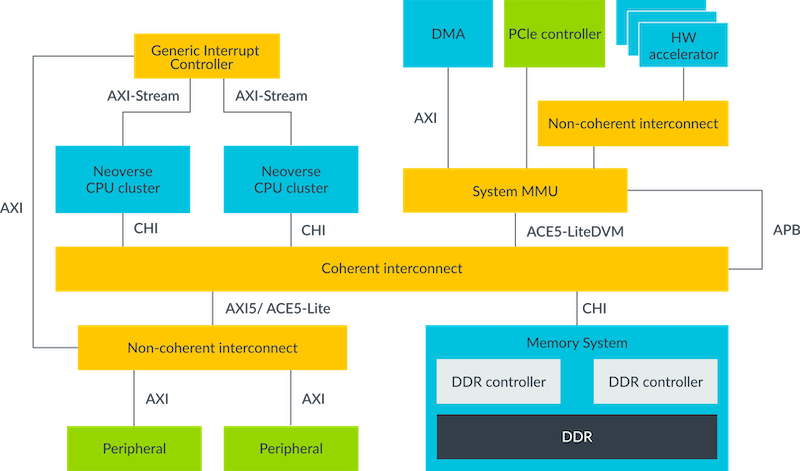
\includegraphics[width=0.7\textwidth]{images/AMBA.png}
    \caption{Diagramma raffigurante SoC, tutti i collegamenti saranno decisi dal protocollo AMBA, si può notare come figura il protocollo AXI\cite{amba}}
    \label{fig:my_label}
\end{figure}
\subsection{Perchè e dov'è usato AMBA}
Il protocollo AMBA è usato per semplificare lo sviluppo di schede contenenti più processori e un grande numero di periferiche e controllori.\\
È diventato uno standard data la sua flessibilità, compatibilità, larghezza di banda e latenza.
\section{Advanced eXtensible Interface}
È un protocollo di interfaccia sviluppato sulle architetture ARM e parte del protocollo AMBA.
\begin{figure}
    \centering
    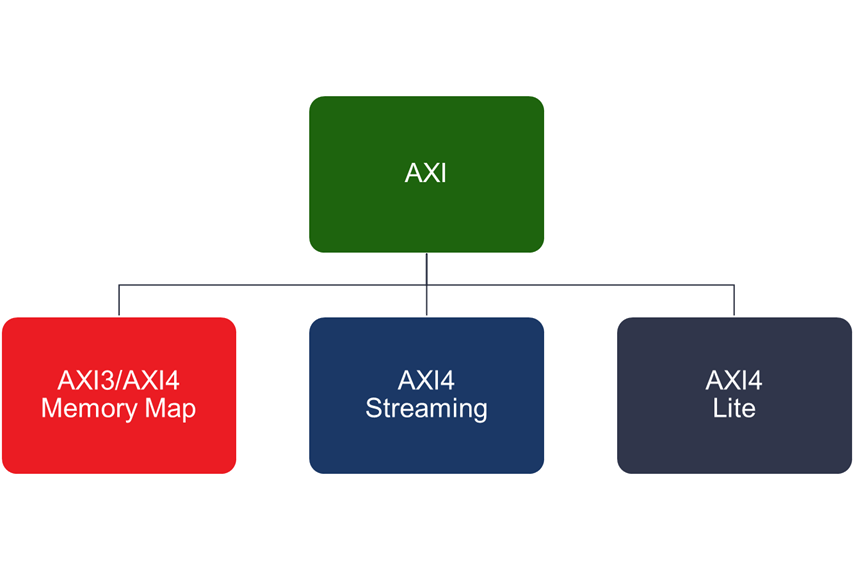
\includegraphics[width=0.5\textwidth]{images/AXI1.png}
    \caption{I 3 tipi d'interfaccia AXI}
    \label{fig:my_label}
\end{figure}
L'AXI è un protocollo master-slave, usato per connessioni con periferiche e memorie, essendo presenti più master in base alle priorità si determina quale master potrà usare il bus, mentre un decodere eseguirà la selezione dello slave.\\
Le operazioni sono eseguite in burst, solitamente da 256bit, che può richiedere più cicli di clock per esser completata, ogni burst consiste in due fasi, la prima di indirizzamento e la seconda di scambio dati, fornendo elevate prestazioni per accessi di tipo memory mapped.\\
È composto da 5 canali indipendenti tra master e slave\cite{AXI} :
\begin{itemize}
    \item Write Address 
    \item Write Data
    \item Read Address
\end{itemize}
Quelli direzione Master to Slave, mentre Slave to Master:
\begin{itemize}
    \item Write Response
    \item Read Data
\end{itemize}
\begin{figure}
    \centering
    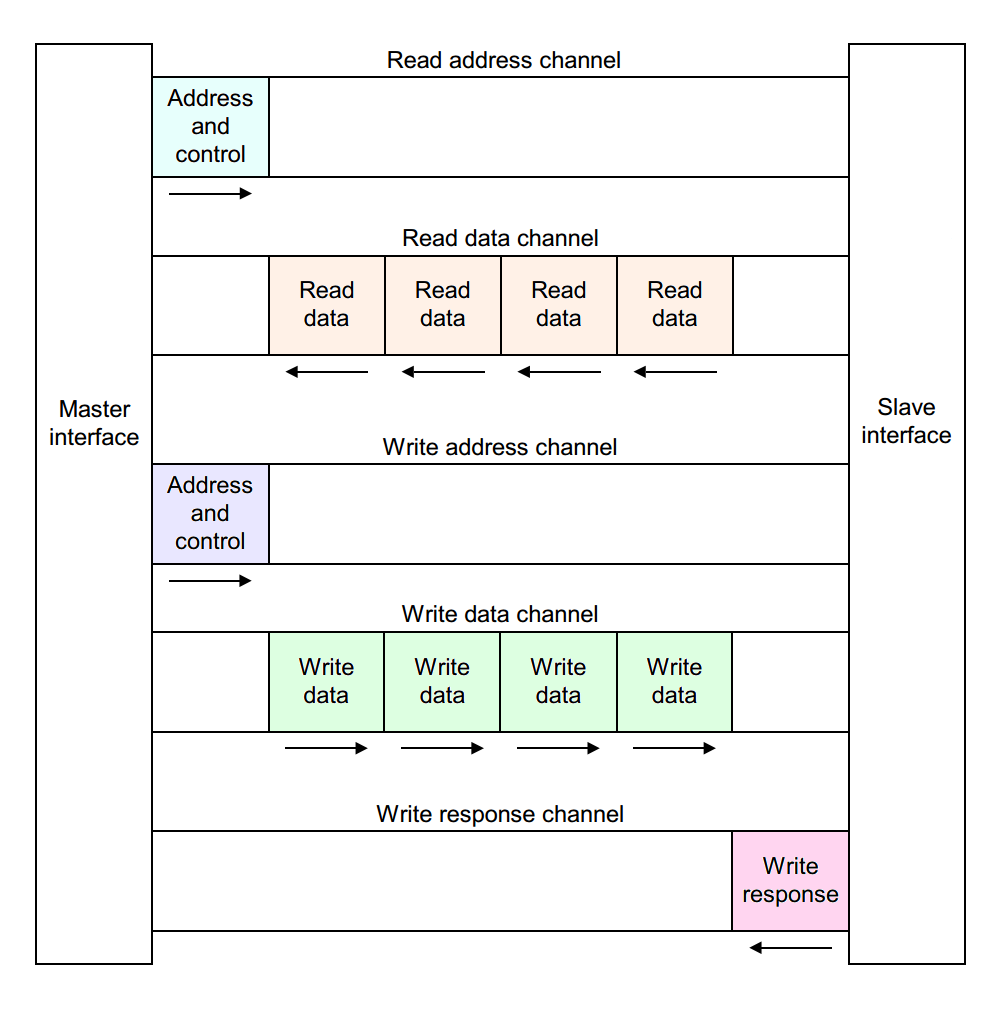
\includegraphics[width=0.9\textwidth]{images/AXI2.jpg}
    \caption{Esempio di comunicazione tramite protocollo AXI, i blocchi multipli stanno ad identificare i Burst}
    \label{fig:my_label}
\end{figure}
I dati possono viaggiare simultaneamente in entrambe le direzioni, esso è possibile per via delle due connessioni separate, in indirizzi e dati, sia per lettura che per scrittura. Ogni scambio di dati è detto transazione essa include l'indirizzo, le informazioni di controllo, i dati inviati e qualsiasi informazione di risposta.
\subsection{AXI nei sistemi ZYNQ}
Nell'architettura ZYNQ-7000, ma come tutte le architetture ZYNQ, il protocollo AXI permette l'interfacciamento tra Processing System (PS) e Programmable Logic (PL).
\begin{figure}
    \centering
    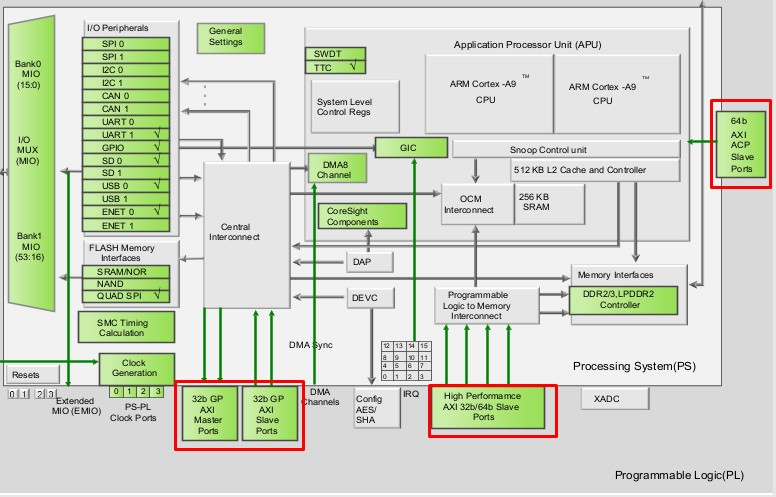
\includegraphics[width=0.9\textwidth]{images/AXI3.jpg}
    \caption{Design di un architettura ZYNQ-7000, dove sono evidenziati i blocchi AXI}
    \label{fig:my_label}
\end{figure}
\begin{figure}
    \centering
    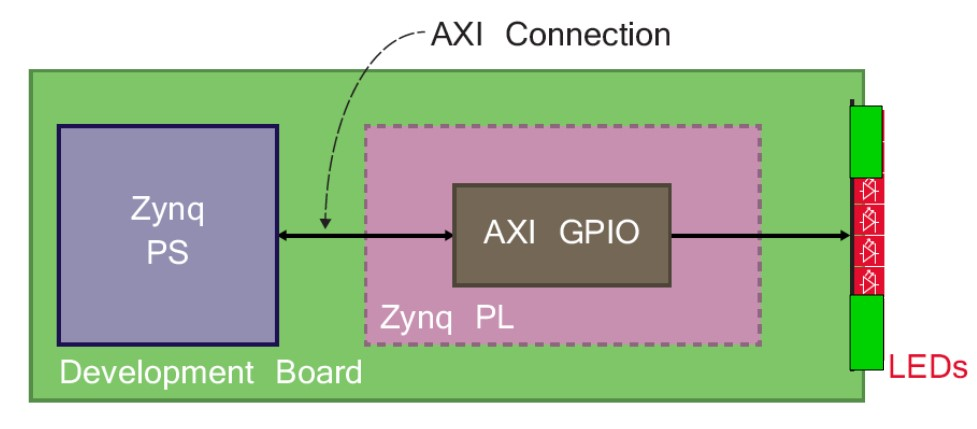
\includegraphics[width=0.7\textwidth]{images/axi.jpg}
    \caption{Zoom della connessione tra PS e PL}
    \label{fig:my_label}
\end{figure}\\
In quest'architettura abbiamo delle interfacce di comunicazione sul bus AXI.
Al fine di facilitare lo sviluppo della scheda la xilnix ha prodotto un componente, completamente riprogrammabile, detto AXI Interconnect, esso facilità e gestisce tutte le connessioni tra master e slave.\clearpage
\begin{figure}
    \centering
    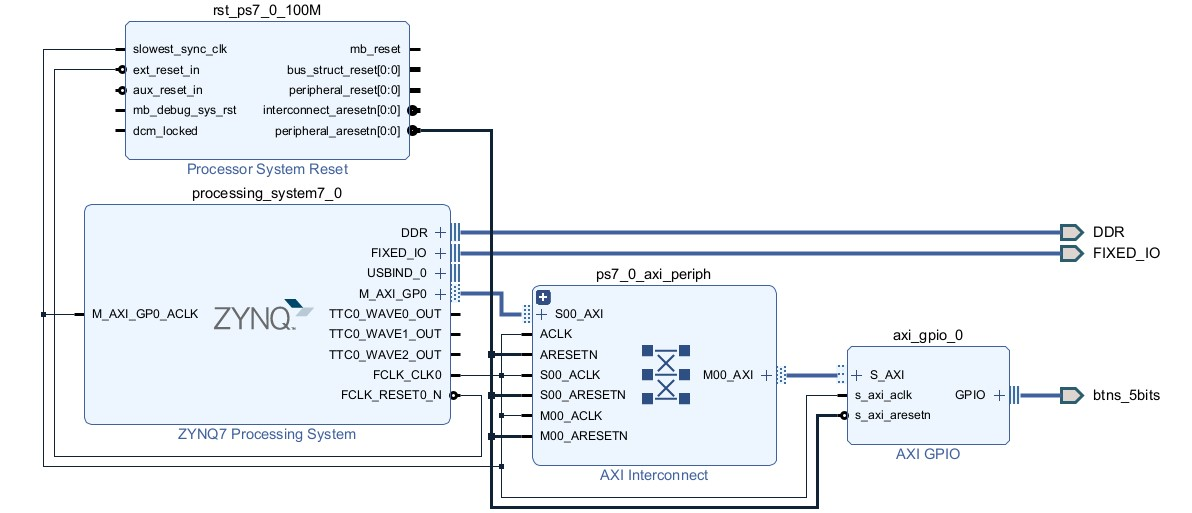
\includegraphics[width=0.9\textwidth]{images/AXI4.jpg}
    \caption{Schema contentente l'interconnecter}
    \label{fig:my_label}
\end{figure}
\subsection{Comunicazione memory-mapped tra PS e PL}
Al fine di far comunicare tramite gli indirizzi definiti in fase di progettazione dobbiamo usare il Central Direct Memory Access (CDMA), esso è un core prodotto da Xilnix che ci permette di avere una connessione tra una sorgente con un indirizzo memory-mapped  ed una destinazione con un indirizzo memory-mapped, tramite il protocollo AXI. Quindi è in grado di associare un indirizzo mappato in memoria fisica con un indirizzo mappato in memoria logica, evitando cosi il vincolo imposto dal sistema operativo sull'accesso agli indirizzi fisici tramite la funzione mmap. \clearpage
\begin{figure}
    \centering
    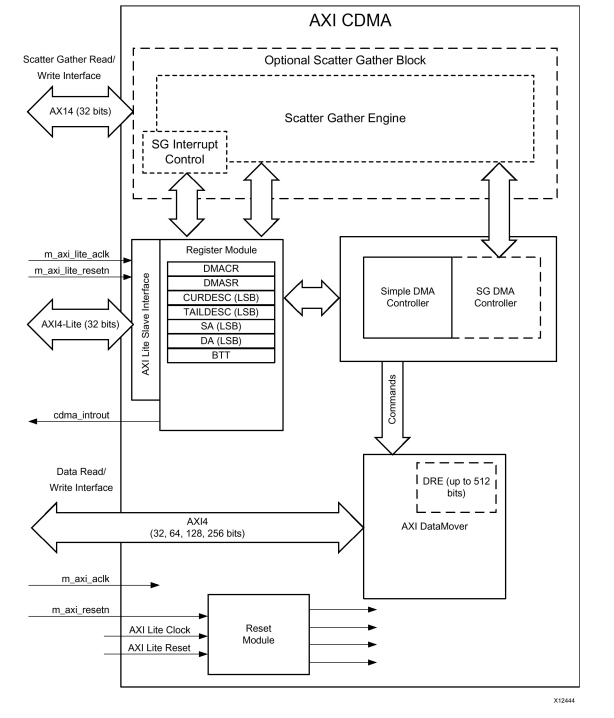
\includegraphics[width=0.8\textwidth]{images/AXI6.jpg}
    \caption{Schema del CDMA}
    \label{fig:my_label}
\end{figure}

Nel caso di un FPGA SoC con un Real Time OS (RTOS), può esser usata per interfacciarsi con il GPIO lato FPGA, con dei core di calcolo tensoriale o per la riprogrammazione sia completa che parziale della PL.
\section{Driver AXI}
Andremo a programmare, leggere e manipolare i dati presenti nella Programmable Logic ed interconnessi con la PS tramite il protocollo AXI e sfruttando il core CDMA ed il funzionamento di esso
\begin{figure}
    \centering
    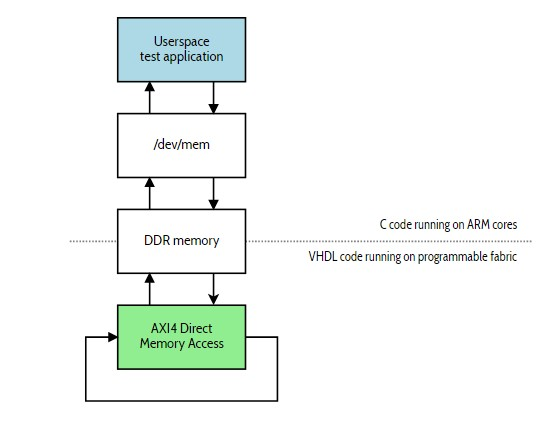
\includegraphics[width=0.7\textwidth]{images/AXI7.jpg}
    \caption{Funzionamento minimo del CDMA}
    \label{fig:my_label}
\end{figure}\\
Il driver necessita di conoscere gli indirizzi base dei core interconnessi al protocollo AXI e la loro dimensione ed eventuale offset.
\begin{lstlisting}[language=C, label=lst:C, caption={Definizione costanti}]
    #define GPIO_BASE_ADDRESS       0x42000000
    #define GPIO_MAP_SIZE           0x1000
    #define XAXIGPIO_DATA_OFFSET    0x00000000
\end{lstlisting}
Poichè necessitiamo di usare \textit{/dev/mem/}, file che rappresenta l'immagine della memoria centrale del microprocessore, per effettuare l'associazione tra indirizzo fisico noto ed indirizzo logico, dobbiamo andare ad effettuare un'apertura assicurandoci che sia andato a buon fine
\begin{lstlisting}[language=C, label=lst:C, caption={Apertura file mem}]
    int memfd;
    if ( (memfd = open("/dev/mem", O_RDWR | O_DSYNC)) == -1 ){
        printf("Can't open /dev/mem.\n");
        exit(-1);
    }
\end{lstlisting}
Una volta effettuato ciò potremmo andare accedere, tramite la funzione mmap all'indirizzo del core AXI con la quale vogliamo interfacciarci, quest'apertura dovra esser sia in lettura che scrittura e map shared, quindi visibile anche a tutti i processi mappati nella stessa regione, quindi usiamo
\begin{lstlisting}[language=C, label=lst:C, caption={Mapping dell'indirizzo di GPIO}]
    void *gpioMapAddr = NULL;
    gpioMapAddr = mmap(0, GPIO_MAP_SIZE, PROT_READ | PROT_WRITE, MAP_SHARED, memfd, GPIO_BASE_ADDRESS);
    if (gpioMapAddr == (void *) -1){
        printf("Can't map the CDMA-Control-Port to user space.\n");
        exit(-1);
    }
\end{lstlisting}
Se il tutto ha avuto esito positivo possiamo effettuare la manipolazione dei dati presenti in esso, andando a sommare l'eventuale offset e l'indirizzo fornitoci dalla funzione mmap
\begin{lstlisting}[language=C, label=lst:C, caption={Esempio con un contatore tramite i led}]
    unsigned long ii;
    for(ii=0; ii<256; ii++){
        *((volatile unsigned long*) (gpioMapAddr + XAXIGPIO_DATA_OFFSET)) = ii;
        printf("led = 0x%02x\n", ii);
        usleep(20000); // sleep 20ms
    }
\end{lstlisting}
Questo esempio può esser modificato ad hoc al fine di accedere ai core interconnessi con il protocollo AXI, questo da la base alla partial reconfiguration tramite due controller già presenti nei SoC. Questo codice può esser compilato sia on-board, sia tramite la cross compilazione, per la cross compilazione si rimanda a \ref{crossComp}\clearpage


